\section{Мульти-агентное обучение с подкреплением}

\subsection{Связь с теорией игр}

Попробуем представить ситуацию, когда в среде действует два агента. Функция переходов теперь зависит от действий каждого из агентов $p(s' \mid s, a^1, a^2)$, а каждый агент оптимизирует свою функцию награды $r^i(s, a^1, a^2)$, где $i$ --- номер агента.

Рассмотрим сеттинг, аналогичный бандитам: игра с одним состоянием, заканчивающаяся после первого выбора. Допустим также детерминированность функций наград. Мы получим в чистом виде задачу, исследующуюся в \emph{теории игр}: заданы две функции $r^1(a^1, a^2), r^2(a^1, a^2)$, зависящие от действий обоих игроков; игроки оптимизируют каждый свою функцию, при этом производя выбор действий одновременно. Отсюда видно, что любой мульти-агентный RL тесно связан с теорией игр: в частности, при обучении агенты могут застрять не только в локальных оптимумах, но и в \href{https://ru.wikipedia.org/wiki/\%D0\%A0\%D0\%B0\%D0\%B2\%D0\%BD\%D0\%BE\%D0\%B2\%D0\%B5\%D1\%81\%D0\%B8\%D0\%B5_\%D0\%9D\%D1\%8D\%D1\%88\%D0\%B0}{\emph{равновесиях Нэша}} (Nash equilibrium), когда ни один другой агент не может поменять свою стратегию в предположении неизменности стратегий других агентов так, чтобы увеличить свою награду.

В общем случае в среде действует $N$ агентов. Будем обозначать как $a^i$ действие $i$-го агента; $\vec{a}$ --- вектор из всех действий всех агентов; $a^{-i}$ --- действия всех агентов, кроме $i$-го. Тогда функция переходов теперь выглядит как $p(s' \mid s, \vec{a})$, а $i$-ый агент оптимизирует свою функцию награды $r^i(s, \vec{a})$. Природа этих функций наград может быть самой разной.

\begin{definition}
Если функции наград всех агентов совпадают, то задача называется \emph{кооперативной}.
\end{definition}

\begin{definition}
Задача с двумя агентами, в которой $r^2(s, \vec{a}) = -r^1(s, \vec{a})$, называется \emph{антагонистической}.
\end{definition}

Это предельные случаи частных ситуаций: если $r^1$ в целом велико там, где велико $r^2$, то агенты, видимо, должны научиться вместе выполнять какую-то задачу. Если же большое $r^1$ влечёт малое $r^2$, то агенты противостоят друг другу. В общем случае у каждого агента может быть какая-то своя задача; этот общий случай иногда называют \emph{смешанной} (mixed) задачей мульти-агентного RL. Зачастую агенты действуют в условиях частичной наблюдаемости, и тогда у каждого агента могут быть свои наблюдения; это означает, что у $i$-го агента своя функция $p^i(o \mid s)$, определяющая наблюдение по текущему состоянию мира. Для простоты далее частичная наблюдаемость опущена. 

\subsection{Централизация обучения}

\emph{Децентрализованный сеттинг} означает, что у агентов нет какой-либо общего <<сервера>> с общими данными, в том числе во время обучения. Простейший подход мульти-агентного RL в рамках такого сеттинга --- завести для каждого агента свою стратегию $\pi^i(a \mid s)$ и оценочную функцию $Q^i(s, a^i)$, которая будет зависеть только от действия $i$-го агента, и оптимизировать их с опыта данного агента любыми обычными RL алгоритмами. Тот факт, что в среде действуют другие агенты, игнорируется. Важный момент: если другие агенты не обучаются (не изменяются с течением времени), то такой подход обучения $i$-го агента корректен.

\begin{proposition}
Если все агенты, кроме $i$-го, стационарны, то $i$-ый агент живёт в MDP с функцией переходов
$$p(s' \mid s, a^i) \coloneqq \int p(s' \mid s, a^i, a^{-i})\pi^{-i}(a^{-i} \mid s) \diff a^{-i},$$
где $\pi^{-i}(a^{-i} \mid s)$ --- стратегия остальных агентов, в предположении их независимого выбора своих действий равная
$$\pi^{-i}(a^{-i} \mid s) \coloneqq \prod_{j \ne i} \pi^j(a^j \mid s)$$
\end{proposition}

Это означает, что если в среде действует другой агент, использующий стационарную стратегию, среда остаётся стационарной и вся теория остаётся справедлива. Однако, если в среде действует другой агент, который обучается (и, значит, меняет свою стратегию с течением времени), то для прочих агентов это означает, что постоянно изменяются <<законы физики>> окружающей среды, и мы под изученную теорию подпадать перестаём. 

В нестационарных средах естественно использовать on-policy обучение. Запуск какого-нибудь on-policy алгоритма с игнорированием факта присутствия других обучающихся агентов обычно оказывается серьёзным бэйзлайном.

\emph{Полностью централизованный сеттинг} возможен для агентов, например, оптимизирующих одну и ту же функцию награды, находящихся в кооперации. Полная централизация означает, что для построения системы из нескольких кооперирующихся агентов все они рассматриваются как единый агент. Наблюдение есть совокупность наблюдений всех агентов, действия --- набор действий для каждого из агентов, и тогда по сути задача сведена к <<одноагентной>> ситуации. В большинстве случаев такой вариант не годится по самой постановке задачи: наличие единого <<центрального сервера>>, который бы принимал решения за всех агентов в среде, может быть просто-напросто очень дорогим. Хотя бы потому что агентов может быть много, и пространство состояний и, главное, действий, взорвётся. В большинстве случаев хочется, чтобы агенты принимали решения на основе только имеющейся у них информации.

Зачастую доступен интересный промежуточный вариант (\emph{частичная централизация}), когда у каждого из кооперирующихся агентов хранится и обучается персональная стратегия, но, например, оценочная функция $Q(s, a^1, a^2 \dots)$ хранится и обучается на общем для всех агентов <<сервере>>. Важно, что эта оценочная функция нужна в on-policy алгоритмах только для обучения, и при использовании полученных стратегий <<сервер>> не потребуется. Это означает, что по окончании обучения в таком сеттинге для использования стратегии никакого центрального сервера не понадобится. Такой подход называется \emph{centralised training with decentralised execution} (CTDE), и многие алгоритмы для мульти-агентного RL строятся именно в рамках этой парадигмы.

В рамках парадигмы CTDE, помимо прочего, возможен \emph{parameter sharing}: если задача симметрична для каких-то агентов, то веса их стратегий считаются общими. Градиенты для их обучения тогда вычисляются на общем сервере; дальше во время использования агенты используют одну и ту же модель для принятия решений. Другими словами, в рамках CTDE подхода при желании обучить колонию из 100 одинаковых муравьёв, вам понадобится лишь одна модель; без частичной централизации же, в децентрализованном сеттинге, подразумевается, что каждый из муравьёв должен как-то сам обучиться, и тогда у каждого из сотни получится в итоге своя модель.

\subsection{Self-play в антагонистических играх}

В симметричных антагонистических играх обучение на опыте игр с самим собой оказалось мощным инструментом. Этот подход называют \emph{self-play}, и заключается он в том, что за обоих игроков играет одна и та же стратегия (такие игры обычно симметричны, и поэтому можно считать, что применяется parameter sharing). Собранный опыт как со стороны одного игрока, так и другого, можно использовать для обучения, и он обладает одним очень ценным свойством: сбалансированностью. На какой бы стадии обучения ни был агент, играет ли он на уровне гранд-мастера или бесконечно сильно тупит, при игре с самим собой в половине случаев он <<выигрывает>>, в половине --- <<проигрывает>>. Разница в сигнале всегда даёт возможность дальнейшего улучшения.

В режиме self-play можно запустить любые алгоритмы обучения: как model-free, так и model-based. В частности, в model-based алгоритмах вроде AlphaGo и MuZero в ходе планирования можно при построении дерева ходы за оппонента проводить при помощи тех же моделей, но не максимизировать, а минимизировать награду. Понятно, что идея применима как в ситуации, когда игроки ходят одновременно, так и когда игроки ходят по очереди (что более типично для игр вроде шахмат и го).

Конечно, self-play не гарантирует, что по итогам обучения стратегия будет способна адаптироваться к произвольному оппоненту. Можно показать, что к обученным self-play методам стратегии можно применить \emph{adversarial-атаку}: зафиксировать её и обучать стратегию оппонента побеждать. Такие стратегии, которые <<взламывают>> стратегию оппонента, зачастую ведут себя очень странно, и могут победить, ничего не делая.

\begin{example}[Adversarial Policy]
По \href{https://adversarialpolicies.github.io/}{данной ссылке} в примерах слева показаны игры стратегии, обученной в режиме self-play. На вид кажется, что полученная стратегия невероятно крута. Далее эта стратегия фиксировалась, и обучалась с нуля новая стратегия оппонента <<побеждать>> фиксированную. Примеры этих игр показаны справа: новая стратегия оппонента просто падает, сбивает с толку <<крутую>> стратегию, и та отправляется в какой-то нокаут.
\end{example}

\subsection{QMix в кооперативных играх}

Рассмотрим кооперативный сеттинг, где все агенты максимизируют одну и ту же функцию награды. Будущую кумулятивную награду после выполнения набора действий $\vec{a}$ в состоянии $s$ для набора политик $\pi^i(a^i \mid s)$ обозначим как $Q^{\mathrm{tot}}(s, \vec{a})$, скаляр. Попробуем построить алгоритм в рамках парадигмы CTDE, то есть обучить <<на центральном сервере>> стратегии $\pi^i(a^i \mid s)$, которые смогут дальше действовать в среде без использования подобного сервера.

Допустим, мы знаем $Q^{\mathrm{tot}}(s, \vec{a})$. Тогда оптимально выбрать действия
$$\argmax_{\vec{a}} Q^{\mathrm{tot}}(s, \vec{a}),$$
однако есть две проблемы. Во-первых, если агентов много, поиск такого аргмаксимума может стать слишком сложной задачей, ровно как и моделирование такой оценочной функции. Во-вторых, в рамках CTDE в частично наблюдаемом сеттинге каждый агент на вход вместо $s$ на самом деле получает своё собственное наблюдение $o^i$ и не знает наблюдения других агентов, когда $Q^{\mathrm{tot}}$ принимает на вход наблюдения всех агентов. С обоими проблемами можно побороться следующим образом.

\begin{definition}
\emph{Смешивающей сетью} (mixing network) назовём моделирование $Q^{\mathrm{tot}}(s, \vec{a})$ в следующем виде:
\begin{equation}\label{vdn}
Q^{\mathrm{tot}}(s, \vec{a}) = Q^{\mathrm{tot}}(Q^1(s, a^1), Q^2(s, a^2), \dots Q^N(s, a^N), s, \phi),
\end{equation}
где $\phi$ --- параметры, $Q^i(s, a^i)$ --- скаляры, зависящие только от той информации, которая доступна $i$-му агенту.
\end{definition}

В частности, в частично наблюдаемом сеттинге $Q^i(s, a^i)$ вместо $s$ принимает на вход наблюдение $i$-го агента $o^i$ и моделируется рекуррентной сетью. Сразу оговоримся, что здесь $Q^i(s, a^i)$, несмотря на принятое обозначение, не является оценочной функцией и не имеет смысл будущей кумулятивной награды. Это лишь некоторая промежуточная вспомогательная величина, через которую по некоторым правилам выражается $Q^{\mathrm{tot}}(s, \vec{a})$, награда <<всей команды>>.

\begin{example}[Value decomposition network] Рассмотрим самый простой пример смешивающей сети, не использующей параметров вовсе:
$$Q^{\mathrm{tot}}(s, \vec{a}) \coloneqq \sum_i Q^i(s, a^i)$$
У этой декомпозиции есть интересное свойство: 
\begin{equation}\label{consistent_vdn}
\argmax_{\vec{a}} Q^{\mathrm{tot}}(s, \vec{a}) = \left[ 
\begin{matrix}
\argmax\limits_{a^1} Q^1(s, a^1) \\
\argmax\limits_{a^2} Q^2(s, a^2) \\
\vdots \\
\argmax\limits_{a^N} Q^N(s, a^N) \\
\end{matrix}
\right]
\end{equation}
\end{example}

Другими словами, будущая награды команды моделируется через какие-то псевдооценочные функции каждого агента команды в отдельности. Нам крайне интересно свойство \eqref{consistent_vdn}.

\begin{definition}
Скажем, что смешивающая сеть \emph{консистентна} (consistent), если для всех состояний выполняется \eqref{consistent_vdn}.
\end{definition}

Консистентность означает, что каждому агенту вовсе не нужно знать наблюдения других агентов или обращаться к центральному серверу для выбора оптимального действия: он берёт лишь значение свой псевдооценочной функции $Q^i(s, a^i)$ и берёт аргмакс по нему. Свойство \eqref{consistent_vdn} гарантирует, что это даст аргмаксимум по всему набору действий $\vec{a}$ всей команды. Поскольку выбор декомпозиции --- наш произвол, нам хочется выбрать такое параметрическое семейство смешивающих сетей, которое гарантирует это свойство. В целом, это не так сложно.

\begin{theorem}
Смешивающая сеть \eqref{vdn} консистентна, если
\begin{equation}\label{qmix_condition}
\frac{\diff Q^{\mathrm{tot}}}{\diff Q^i} \ge 0,
\end{equation}
то есть для всех состояний $s$ и при любых значениях параметров $\phi$ награда команды монотонно зависит от псевдооценочной функции $Q^i(s, a^i)$.
\begin{proof}
В силу монотонности, для любых действий $\vec{a}$:
$$Q^{\mathrm{tot}}( \max_{a^1} Q^1(s, a^1), \dots \max_{a^N} Q^N(s, a^N), s, \phi) \ge Q^{\mathrm{tot}}( Q^1(s, a^1), \dots Q^N(s, a^N), s, \phi),$$
следовательно максимизация всех аргументов монотонной функции максимизирует саму функцию.
\end{proof}
\end{theorem}

Можно ли придумать какое-нибудь богатое семейство смешивающих сетей с параметрами, для которых было бы выполнено \eqref{qmix_condition}? Давайте возьмём нейросеть с параметрами $\phi$, которая принимает на вход скаляры $Q^1(s, a^1), \dots Q^N(s, a^N)$ и выдаёт скаляр $Q^{\mathrm{tot}}$. Тогда:
\begin{proposition}
Пусть нейросеть полносвязная, состоит из чередования линейных слоёв и монотонных функций активаций, и все параметры нейросети $\phi_i$ (кроме, возможно, смещений в линейных слоях) неотрицательны. Тогда выполнено \eqref{qmix_condition}.
\begin{proof}
Композиция монотонных преобразований монотонно; линейная комбинация с положительными весами (и произвольными смещениями) также монотонно не убывает как функция от входов.
\end{proof}
\end{proposition}

Итак, любая нейросеть с положительными весами подходит нам в качестве смешивающей. Сделаем ещё одно наблюдение: эта нейросетка очень маленькая, ведь на вход ей подаётся вектор размерности $N$, где $N$ --- число агентов, а на выходе скаляр. Заметим также, что веса могут зависеть от состояния: мы можем использовать разные $\phi$ для разных состояний $s$, и отсюда возникает идея, как можно повысить гибкость нашей value decomposition network.

\begin{definition}
\emph{Гиперсетью} (hypernetwork) называется нейросеть, выдающая веса для другой нейросети.
\end{definition}

Мы заведём гиперсеть $\phi(s, \theta)$, которая для данного состояния $s$ будет с параметрами $\theta$ выдавать на центральном сервере веса для смешивающей сети. В частности, $\phi(s, \theta)$ уже не обязано быть монотонным и может моделироваться произвольной обычной нейросетью. Мы получим, что в каждом состоянии у нас есть какое-то своё монотонное преобразование псевдооценочных функций каждого агента в оценочную функцию команды, и это очень удобно.

Итого в алгоритме QMIX оценочная функция моделируется в следующем виде:
$$Q^{\mathrm{tot}}(s, \vec{a}, \theta, \phi) \coloneqq Q^{\mathrm{tot}}( Q^1(s, a^1, \psi^1), \dots Q^N(s, a^N, \psi^N), \phi(s, \theta)),$$
где $\psi^i$ --- параметры псевдооценочной функции (возможен parameter sharing, если задача симметрична для некоторых агентов), $\theta$ --- параметры гиперсети, $\phi(s, \theta)$ --- получающиеся параметры смешивающей нейросети.

Процесс обучения стандартный и похож на обычный DQN. При взаимодействии со средой $i$-ый агент использует свою псевдооценочную функцию $Q^i(s, a^i)$ и ведёт себя $\eps$-жадно. Собранные переходы $(s, \vec{a}, r, s')$ собираются на центральном сервере. Для перехода $\T \coloneqq (s, \vec{a}, \vec{r}, s')$ целевая переменная строится как 
$$y(\T) \coloneqq r + \gamma \max_{\vec{a}'} Q^{\mathrm{tot}}(s', \vec{a}', \theta^-, \phi^-),$$
где $\theta^-, \phi^-$ --- замороженные параметры таргет-сети. Далее с таким таргетом минимизируется MSE по всем параметрам:
$$\E_\T (y(\T) - Q^{\mathrm{tot}}(s, \vec{a}, \theta, \phi))^2 \to \min_{\theta, \phi}$$
После окончания обучения центральный сервер, на котором хранится гиперсеть и смешивающая сеть, не нужны, и агенты используют лишь локальные певдооценочные функции $Q^i(s, a^i)$.

\subsection{Multi-Agent DDPG (MADDPG) в смешанных играх}

Рассмотрим смешанную игру, где функции наград агентов произвольны. На <<центральном сервере>> будем хранить общую оценочную функцию, которая теперь должна выдавать будущие награды сразу для всех агентов. 

\begin{definition}
При данных политиках $\pi^j(a_j \HM\mid s)$ \emph{централизованной оценочной функцией} (centralized state-action value function)  обозначим $\vec{Q}(s, \vec{a})$, возвращающую вектор, $i$-ая компонента которого $Q^i(s, \vec{a})$ равна будущей кумулятивной награде, которую получит $i$-ый агент после выполнения набора действий $\vec{a}$ в состоянии $s$.
\end{definition}

На центральном сервере понятно, как учить такую Q-функцию, причём это можно делать в off-policy режиме. Для произвольного перехода из буфера $\T \coloneqq (s, \vec{a}, \vec{r}, s')$ строим таргет
$$y(\T) \coloneqq \vec{r} + \gamma \vec{Q}(s', \vec{a}'),$$
где $\vec{a}'$ порождены оцениваемыми $\pi^j(a'_j \HM\mid s')$ (для стабилизации процесса --- таргет-сетями для них), и минимизируем стандартное MSE:
$$\E_\T (\vec{Q}(s, \vec{a}) - y(\T))^2 \to \min_{\vec{Q}}$$

Процесс необходимо проводить на центральном сервере, поскольку для вычисления таргета необходимы текущие стратегии всех агентов. Вообще, от этого ограничения можно избавиться, если агентам в их наблюдениях доступны действия всех остальных агентов. Тогда мы сможем перейти к децентрализованному обучению следующим образом: $i$-ый агент может локально хранить и обучать лишь интересующую его компоненту $Q^i(s, \vec{a})$. При построении таргета нужны стратегии опонентов; их $i$-ый агент будет \emph{моделировать}. Для моделирования собираются наблюдения $(s, a^{-i})$, то есть какие действия предприняли остальные агенты в состоянии $s$, и дальше агент учится предсказывать действия других игроков по этой обучающей выборке в supervised-режиме:
$$\E_{s, a^{-i}} \log \mu(a^{-i} \mid s) \to \max_{\mu},$$
обычно с добавлением энтропийного регуляризатора. Имея такое приближение стратегий оппонентов на руках, таргет для обучения критика рассчитывается по формуле
$$y^i(\T) \coloneqq r^i + Q^i(s', a'^i, a'^{-i}),$$
где $a'^i \HM\sim \pi^i(a'^i \mid s')$, а $a'^{-i} \sim \mu(a'^{-i} \mid s')$.

Как использовать централизованную оценочную функцию для обучения актёров? Для обучения $i$-го актёра с параметрами $\theta^i$ можно применить формулу policy gradient:
\begin{equation}\label{MAPG}
\nabla_{\theta^i} = \E_{s} \E_{a^i \sim \pi^i(a^i \mid s)} \nabla_{\theta^i} \log \pi^i(a_i \HM\mid s) Q^i(s, a^i, a^{-i})
\end{equation}
Действительно, для формулы градиентов по $\theta^i$ остальные стратегии можно считать фиксированными; поэтому стандартная формула применима. В ней состояния $s$ приходят из опыта взаимодействия агентов со средой, а действия других агентов $a^{-i}$ должны быть порождены этими самыми стратегиями прочих агентов. 

Авторы MADDPG предлагают перейти здесь от policy gradient-схемы к использованию формулы аля DDPG, и забить на частоты посещения состояний. Тогда в формуле \eqref{MAPG} можно брать $s$, $a^{-i}$ --- из приближения стратегий других агентов. По аналогии с DDPG также можно обучать детерминированную стратегию $\pi^i(s)$ с параметрами $\theta^i$, оптимизируя
$$\E_{s} \E_{a^i} Q^i(s, \pi^i(s), a^{-i}) \to \max_{\theta^i},$$
где $s$ берутся из реплей буфера, $a^{-i}$ моделируются или, в случае CTDE-обучения, берутся из честных стратегий $\pi^j(s), j \HM\ne i$; в последнем случае мат.ожидание по $a^{-i}$ вырождается.

\subsection{Системы коммуникации (DIAL)}

Пожалуй, главной особенностью взаимодействия агентов вроде людей в природе является такое явление, как язык. Давайте попробуем в парадигме RL промоделировать, как агенты могут передавать друг другу сообщения.

\begin{definition}
Скажем, что у агента $i$ есть \emph{канал связи} (communication channel), если на каждом шаге агент помимо действия $a^i$ выбирает некоторое \emph{сообщение} (message) $m^i$, которое не влияет на функцию переходов и функции награды, и которое все агенты получают вместе со своими наблюдениями на следующем шаге.
\end{definition}

Конечно, можно обобщить это понятие и сказать, что канал связи есть между конкретными агентами $i, j$, и этот канал может быть односторонним, двухсторонним, и так далее, но нам это сейчас не принципиально. Мы можем использовать эту идею в произвольных мульти-агентных средах, в том числе обучая агентов децентрализованно, рассматривая $m^i$ как часть пространства действий агентов.

\begin{remark}
В таком подходе удобно выбрать дискретное пространство сообщений, а при моделировании Q-функции вместо того, чтобы выдавать оценку для каждой пары действий $(a^i, m^i)$ отдельно выдаются оценки для $a^i$ и отдельно для $\mu^i$; дальше агент $\eps$-жадно выбирает действие для среды и отдельно $\eps$-жадно выбирает сообщение для отправки. Это небольшая декомпозиция упрощает пространство действий.
\end{remark}

Рассмотрим чуть более хитрое применение канала связи под названием Differentiable Inter-Agent Learning (DIAL), применимое для кооперативных задач (с единой функцией награды) в парадигме CTDE. Здесь естественно выбрать непрерывное пространство сообщений. На центральном сервере во время обучения просто заметим, что любые модели агента $j$, на шаге $t$ минимизирующие свои стандартные функции потерь, дифференцируемы по входным наблюдениям и в том числе по полученным от других агентов сообщениям $\mu^i_{t-1}$. Эту информацию о градиенте можно использовать для обучения $i$-го агента выдавать хорошие сообщения! Концептуально, схема для двух агентов в условиях частичной наблюдаемости выглядит примерно так:

\begin{center}
    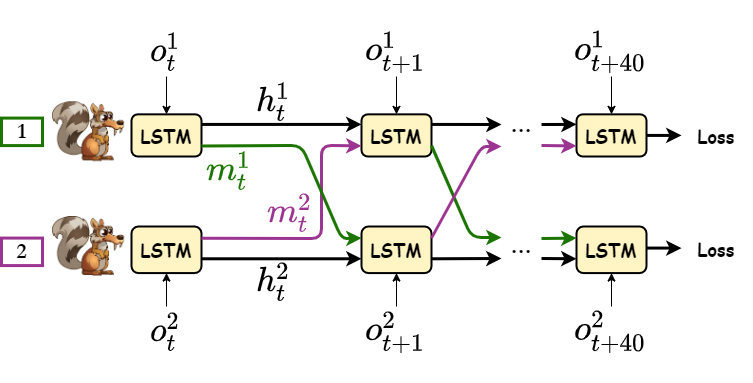
\includegraphics[width=0.65\textwidth]{Images/Communication.png}
\end{center}

На рисунке $o_t^i$ --- наблюдение, поступающее на вход $i$-му агенту на шаге $t$. Оно обрабатывается рекуррентной сетью, которое выдаёт, помимо оценочных функций и вероятностей действий, скрытое состояние $h^i_{t}$ для передачи самому себе на следующий шаг и сообщение $m^i_t$ для передачи другим агентам на следующий шаг (как видно на схеме, между этими двумя сущностями практически нет никакой разницы). Далее это сообщение поступает на вход моделям всех других агентов на шаге $t + 1$. В конце вычислений вычисляется некоторая функция потерь в зависимости от используемого алгоритма (например, MSE для оценочных функций или суррогатная функция потерь для обучения стратегии), и этот градиент проходит не только назад по времени, но и по каналам связи в модели других агентов: как видно, вся эта схема end-to-end дифференцируема.
